% GENERATED FILE - do not hand-edit.
% Source of truth: data/calculus-reviewed/t-8.json in the zenith-website repo.
% Regenerate with: python3 scripts/build_calculus_tex.py
\documentclass[11pt]{article}
\usepackage[utf8]{inputenc}
\usepackage[T1]{fontenc}
\usepackage{amsmath,amssymb}
\usepackage{graphicx}
\usepackage[margin=1in]{geometry}
\graphicspath{{../..//}}
\setlength{\parindent}{0pt}
\setlength{\parskip}{0.6em}
\begin{document}
\section*{Chapter 8: Further Applications of Integration --- Test T8}

\bigskip\noindent\textbf{T1.}\ A particle moves along a line in such a way that its position at time $t$ is given by $s=t^3-9t^2+24t+5$. Its direction of motion changes when
\begin{list}{}{\setlength{\leftmargin}{3em}\setlength{\labelwidth}{2.5em}\setlength{\itemsep}{0pt}\setlength{\topsep}{2pt}}
\item[(A)] $t=2$ only
\item[(B)] $t=4$ only
\item[(C)] $t=6$ only
\item[(D)] $t=2$ and $t=4$
\end{list}

\bigskip\noindent\textbf{T2.}\ A body moves along a straight line so that its velocity $v$ at time $t$ is given by $v=6t^3+4t^2+7$. The distance the body covers from $t=0$ to $t=3$ equals
\begin{list}{}{\setlength{\leftmargin}{3em}\setlength{\labelwidth}{2.5em}\setlength{\itemsep}{0pt}\setlength{\topsep}{2pt}}
\item[(A)] $178.5$
\item[(B)] $157$
\item[(C)] $134$
\item[(D)] $196$
\end{list}

\bigskip\noindent\textbf{T3.}\ A particle moves along a line with velocity $v=4t^2-8t$. The total distance traveled from $t=0$ to $t=4$ equals
\begin{list}{}{\setlength{\leftmargin}{3em}\setlength{\labelwidth}{2.5em}\setlength{\itemsep}{0pt}\setlength{\topsep}{2pt}}
\item[(A)] $0$
\item[(B)] $16$
\item[(C)] $32$
\item[(D)] $48$
\end{list}

\bigskip\noindent\textbf{T4.}\ A particle moves along a line with velocity $v(t)=4t^2-8t$. The net change in position of the particle from $t=0$ to $t=4$ is
\begin{list}{}{\setlength{\leftmargin}{3em}\setlength{\labelwidth}{2.5em}\setlength{\itemsep}{0pt}\setlength{\topsep}{2pt}}
\item[(A)] $0$
\item[(B)] $\dfrac{16}{3}$
\item[(C)] $\dfrac{32}{3}$
\item[(D)] $\dfrac{64}{3}$
\end{list}

\bigskip\noindent\textbf{T5.}\ The acceleration of a particle moving on a straight line is given by $a=2\cos t$, and when $t=0$ the particle is at rest. The distance it covers from $t=0$ to $t=2$ is
\begin{list}{}{\setlength{\leftmargin}{3em}\setlength{\labelwidth}{2.5em}\setlength{\itemsep}{0pt}\setlength{\topsep}{2pt}}
\item[(A)] $2\sin 2$
\item[(B)] $2(1-\cos 2)$
\item[(C)] $2-2\sin 2$
\item[(D)] $-2\cos 2$
\end{list}

\bigskip\noindent\textbf{T6.}\ During the worst 5-hour period of a hurricane the wind velocity, in miles per hour, is given by $v(t)=6t-t^2+120$, $0\leq t \leq 5$. The average wind velocity during this period (in mph) is
\begin{list}{}{\setlength{\leftmargin}{3em}\setlength{\labelwidth}{2.5em}\setlength{\itemsep}{0pt}\setlength{\topsep}{2pt}}
\item[(A)] $120$
\item[(B)] $126\dfrac{2}{3}$
\item[(C)] $130\dfrac{1}{3}$
\item[(D)] $133\dfrac{1}{3}$
\end{list}

\bigskip\noindent\textbf{T7.}\ The acceleration of an object in motion is given by the vector $\vec{a}(t)=\langle 3t, e^{2t}\rangle$. If the object's initial velocity was $\vec{v}(0)=\langle 3,0\rangle$, which is the velocity vector at any time $t$?
\begin{list}{}{\setlength{\leftmargin}{3em}\setlength{\labelwidth}{2.5em}\setlength{\itemsep}{0pt}\setlength{\topsep}{2pt}}
\item[(A)] $\vec{v}(t)=\left\langle \dfrac{3}{2}t^2, \dfrac{1}{2}e^{2t}+1\right\rangle$
\item[(B)] $\vec{v}(t)=\left\langle \dfrac{3}{2}t^2+3, \dfrac{1}{2}e^{2t}\right\rangle$
\item[(C)] $\vec{v}(t)=\left\langle \dfrac{3}{2}t^2+3, \dfrac{1}{2}(e^{2t}-1)\right\rangle$
\item[(D)] $\vec{v}(t)=\langle 3, e^{2t}-1\rangle$
\end{list}

\bigskip\noindent\textbf{T8.}\ A stone is thrown upward from the ground with an initial velocity of 120 ft/sec. Its average velocity (given that $a(t)=-32$ ft/sec$^2$) during the first 3 seconds is
\begin{list}{}{\setlength{\leftmargin}{3em}\setlength{\labelwidth}{2.5em}\setlength{\itemsep}{0pt}\setlength{\topsep}{2pt}}
\item[(A)] $24$ ft/sec
\item[(B)] $48$ ft/sec
\item[(C)] $72$ ft/sec
\item[(D)] $96$ ft/sec
\end{list}

\bigskip\noindent\textbf{T9.}\ Assume that the density of vehicles (number of cars per mile) during morning rush hour, for the 30-mile stretch along a state highway southbound from a bridge, is given by $f(x)$, where $x$ is the distance, in miles, south of the bridge. Which of the following gives the number of vehicles (on this 30-mile stretch) from the bridge to a point $x$ miles south of the bridge?
\begin{list}{}{\setlength{\leftmargin}{3em}\setlength{\labelwidth}{2.5em}\setlength{\itemsep}{0pt}\setlength{\topsep}{2pt}}
\item[(A)] $\displaystyle\int_0^x f(t)\,dt$
\item[(B)] $\displaystyle\int_x^{30} f(t)\,dt$
\item[(C)] $\displaystyle\int_0^{30} f(x)\,dx$
\item[(D)] $\displaystyle\sum_{k=1}^n f(x_k)\,\Delta x$ (where the 30-mile stretch has been partitioned into $n$ equal subintervals)
\end{list}

\bigskip\noindent\textbf{T10.}\ The center of a city, that we will assume is circular, is on a straight highway (along the diameter of the circle). The radius of the city is 5 miles. The density of the population, in thousands of people per square mile, is given by $f(x)=15-3x$ at a distance $x$ miles from the highway. The population of the city (in thousands of people) is given by the integral
\begin{list}{}{\setlength{\leftmargin}{3em}\setlength{\labelwidth}{2.5em}\setlength{\itemsep}{0pt}\setlength{\topsep}{2pt}}
\item[(A)] $\displaystyle\int_0^5 (15-3x)\,dx$
\item[(B)] $\displaystyle 2\int_0^5 (15-3x)\sqrt{25-x^2}\,dx$
\item[(C)] $\displaystyle 4\int_0^5 (15-3x)\sqrt{25-x^2}\,dx$
\item[(D)] $\displaystyle\int_0^5 2\pi x(15-3x)\,dx$
\end{list}

\bigskip\noindent\textbf{TB1.}\ A car accelerates from 0 to 90 mph in 12 seconds, with constant acceleration. (Note that 60 mph = 88 ft/sec, so 90 mph = 132 ft/sec.) The acceleration (in ft/sec$^2$) is
\begin{list}{}{\setlength{\leftmargin}{3em}\setlength{\labelwidth}{2.5em}\setlength{\itemsep}{0pt}\setlength{\topsep}{2pt}}
\item[(A)] $2.2$
\item[(B)] $6.6$
\item[(C)] $8.8$
\item[(D)] $11$
\end{list}

\bigskip\noindent\textbf{TB2.}\ A particle has velocity $\mathbf v(t)=\langle2t,t-2\rangle$ and initial position $(0,2)$. At time $t$ the position vector $\mathbf{R}$ is
\begin{list}{}{\setlength{\leftmargin}{3em}\setlength{\labelwidth}{2.5em}\setlength{\itemsep}{0pt}\setlength{\topsep}{2pt}}
\item[(A)] $\left\langle t^2, -\dfrac{4-t^2}{2}\right\rangle$
\item[(B)] $\left\langle t^2, \dfrac{4-t^2}{2}\right\rangle$
\item[(C)] $\left\langle t^2, \dfrac{t^2-4t}{2}\right\rangle$
\item[(D)] $\left\langle t^2, \dfrac{t^2-4t+4}{2}\right\rangle$
\end{list}

\bigskip\noindent\textbf{TB3.}\ A particle has velocity $\mathbf v(t)=\langle2t,t-2\rangle$ and initial position $(0,2)$. The acceleration vector at time $t=3$ is
\begin{list}{}{\setlength{\leftmargin}{3em}\setlength{\labelwidth}{2.5em}\setlength{\itemsep}{0pt}\setlength{\topsep}{2pt}}
\item[(A)] $\langle 2,1\rangle$
\item[(B)] $\langle 1,-1\rangle$
\item[(C)] $\langle 1,2\rangle$
\item[(D)] $\langle 2,-1\rangle$
\end{list}

\bigskip\noindent\textbf{TB4.}\ A particle has velocity $\mathbf v(t)=\langle2t,t-2\rangle$ and initial position $(0,2)$. The speed of the particle is at a minimum when $t$ equals
\begin{list}{}{\setlength{\leftmargin}{3em}\setlength{\labelwidth}{2.5em}\setlength{\itemsep}{0pt}\setlength{\topsep}{2pt}}
\item[(A)] $0$
\item[(B)] $\dfrac{2}{5}$
\item[(C)] $1$
\item[(D)] $\dfrac{8}{5}$
\end{list}

\bigskip\noindent\textbf{TB5.}\ A particle moves along a curve in such a way that its position vector and velocity vector are perpendicular at all times. If the particle passes through the point $(6,4)$, then the equation of the curve is
\begin{list}{}{\setlength{\leftmargin}{3em}\setlength{\labelwidth}{2.5em}\setlength{\itemsep}{0pt}\setlength{\topsep}{2pt}}
\item[(A)] $x^2+y^2=10$
\item[(B)] $x^2+y^2=52$
\item[(C)] $x^2+2y^2=68$
\item[(D)] $x^2-y^2=20$
\end{list}

\bigskip\noindent\textbf{TB6.}\ The velocity of an object is given by $\vec{v}(t)=\langle 4\sqrt{t}, 6\rangle$. If this object is at the origin when $t=1$, where was it at $t=0$?
\begin{list}{}{\setlength{\leftmargin}{3em}\setlength{\labelwidth}{2.5em}\setlength{\itemsep}{0pt}\setlength{\topsep}{2pt}}
\item[(A)] $\left(-\dfrac{8}{3},-6\right)$
\item[(B)] $\left(\dfrac{8}{3},6\right)$
\item[(C)] $\left(\dfrac{4}{3},0\right)$
\item[(D)] $\left(-\dfrac{4}{3},0\right)$
\end{list}

\bigskip\noindent\textbf{TB7.}\ Suppose the current world population is 10 billion and the population $t$ years from now is estimated to be $P(t)=10e^{0.008t}$ billion people. On the basis of this supposition, the average population of the world, in billions, over the next 30 years will be approximately
\begin{list}{}{\setlength{\leftmargin}{3em}\setlength{\labelwidth}{2.5em}\setlength{\itemsep}{0pt}\setlength{\topsep}{2pt}}
\item[(A)] $9.5$
\item[(B)] $10.8$
\item[(C)] $11.302$
\item[(D)] $12.6$
\end{list}

\bigskip\noindent\textbf{TB8.}\ A beach opens at 8 A.M.\ and people arrive at a rate of $R(t)=15+50t$ people per hour, where $t$ represents the number of hours the beach has been open. Assuming no one leaves before noon, at what time will there be 130 people there?
\begin{list}{}{\setlength{\leftmargin}{3em}\setlength{\labelwidth}{2.5em}\setlength{\itemsep}{0pt}\setlength{\topsep}{2pt}}
\item[(A)] $9{:}45$
\item[(B)] $10{:}00$
\item[(C)] $10{:}15$
\item[(D)] $10{:}30$
\end{list}

\bigskip\noindent\textbf{TB9.}\ Suppose the amount of a drug in a patient's bloodstream $t$ hours after intravenous administration is $A(t)=\dfrac{45}{(t+1)^2}$ mg. The average amount in the bloodstream during the first 5 hours is
\begin{list}{}{\setlength{\leftmargin}{3em}\setlength{\labelwidth}{2.5em}\setlength{\itemsep}{0pt}\setlength{\topsep}{2pt}}
\item[(A)] $6.0$ mg
\item[(B)] $7.5$ mg
\item[(C)] $11.0$ mg
\item[(D)] $16.6$ mg
\end{list}

\bigskip\noindent\textbf{TB10.}\ A rumor spreads through a town at the rate of $R(t)=t^2+15t$ new people per day $t$ days after it was first heard. Approximately how many people hear the rumor during the third week (from the 14th to the 21st days) after it was first heard?
\begin{list}{}{\setlength{\leftmargin}{3em}\setlength{\labelwidth}{2.5em}\setlength{\itemsep}{0pt}\setlength{\topsep}{2pt}}
\item[(A)] $2219$
\item[(B)] $3161$
\item[(C)] $4010$
\item[(D)] $4750$
\end{list}

\bigskip\noindent\textbf{TB11.}\ Oil is leaking from a tanker at the rate of $L(t)=1500e^{-0.4t}$ gal/hr, where $t$ is given in hours. The total number of gallons of oil that will leak out during the first 6 hours is approximately
\begin{list}{}{\setlength{\leftmargin}{3em}\setlength{\labelwidth}{2.5em}\setlength{\itemsep}{0pt}\setlength{\topsep}{2pt}}
\item[(A)] $1271$
\item[(B)] $3031$
\item[(C)] $3410$
\item[(D)] $4323$
\end{list}

\bigskip\noindent\textbf{TB12.}\ Population density depends on distance $x$ from the city center according to $\begin{array}{c|rrrrrr}x\text{ (miles)}&0&3&6&9&12&15\\\hline f(x)\text{ (hundreds per square mile)}&60&50&42&30&18&8\end{array}$. Using the five width3 intervals in the table, apply a left Riemann sum to $100\int_0^{15}2\pi x f(x)\,dx$ to estimate the population, rounded to the nearest person.
\begin{list}{}{\setlength{\leftmargin}{3em}\setlength{\labelwidth}{2.5em}\setlength{\itemsep}{0pt}\setlength{\topsep}{2pt}}
\item[(A)] $60{,}000$
\item[(B)] $376{,}000$
\item[(C)] $691{,}200$
\item[(D)] $1{,}673{,}841$
\end{list}

\bigskip\noindent\textbf{TB13.}\ If a factory continuously dumps pollutants into a river at the rate of $p(t)=\dfrac{\sqrt{t}}{240}$ tons per day, then the amount dumped after 9 weeks is approximately
\begin{list}{}{\setlength{\leftmargin}{3em}\setlength{\labelwidth}{2.5em}\setlength{\itemsep}{0pt}\setlength{\topsep}{2pt}}
\item[(A)] $0.07$ ton
\item[(B)] $0.90$ ton
\item[(C)] $1.39$ tons
\item[(D)] $1.55$ tons
\end{list}

\bigskip\noindent\textbf{TB14.}\ A roast at $180^\circ$F is put into a refrigerator whose temperature is $45^\circ$F. The temperature of the roast is cooling at time $t$ at the rate of $R(t)=-10e^{-0.1t}\,{}^\circ$F per minute. The temperature, to the nearest degree F, of the roast 25 minutes after it is put into the refrigerator is
\begin{list}{}{\setlength{\leftmargin}{3em}\setlength{\labelwidth}{2.5em}\setlength{\itemsep}{0pt}\setlength{\topsep}{2pt}}
\item[(A)] $45^\circ$
\item[(B)] $70^\circ$
\item[(C)] $81^\circ$
\item[(D)] $88^\circ$
\end{list}

\bigskip\noindent\textbf{TB15.}\ How long will it take to release 9 tons of pollutant if the rate at which the pollutant is being released is $P(t)=te^{-0.25t}$ tons per week?
\begin{list}{}{\setlength{\leftmargin}{3em}\setlength{\labelwidth}{2.5em}\setlength{\itemsep}{0pt}\setlength{\topsep}{2pt}}
\item[(A)] $6.8$ weeks
\item[(B)] $7.5$ weeks
\item[(C)] $8.9$ weeks
\item[(D)] $10.2$ weeks
\end{list}

\bigskip\noindent\textbf{TB16.}\ What is the total area bounded by the curve $f(x)=x^3-5x^2+4x$ and the $x$-axis on the interval $0\leq x \leq 4$?
\begin{list}{}{\setlength{\leftmargin}{3em}\setlength{\labelwidth}{2.5em}\setlength{\itemsep}{0pt}\setlength{\topsep}{2pt}}
\item[(A)] $-\dfrac{71}{6}$
\item[(B)] $\dfrac{71}{6}$
\item[(C)] $12$
\item[(D)] $\dfrac{71}{3}$
\end{list}

\bigskip\noindent\textbf{TB17.}\ A tank has signed outward flow rate $W(t)=-0.15t^2-0.4t+3$ gal/hr, where negative values represent inflow. What is the net water loss, in gallons, over $0\le t\le4$?
\begin{list}{}{\setlength{\leftmargin}{3em}\setlength{\labelwidth}{2.5em}\setlength{\itemsep}{0pt}\setlength{\topsep}{2pt}}
\item[(A)] $4.9$
\item[(B)] $5.2$
\item[(C)] $5.6$
\item[(D)] $5.9$
\end{list}

\bigskip\noindent\textbf{TB18.}\ A bacterial culture is growing at the rate of $B(t)=1500e^{0.04t}$ bacteria in $t$ hours. The total increase in bacterial population during the second hour is approximately
\begin{list}{}{\setlength{\leftmargin}{3em}\setlength{\labelwidth}{2.5em}\setlength{\itemsep}{0pt}\setlength{\topsep}{2pt}}
\item[(A)] $1015$
\item[(B)] $1046$
\item[(C)] $1593$
\item[(D)] $1650$
\end{list}

\bigskip\noindent\textbf{TB19.}\ A website opens at noon. Its rate $R(t)$ in visitors/hour increases as shown in the graph, where $t$ is hours after noon. Each vertical grid interval represents one hour, from $t=0$ to $t=8$. Use a midpoint or trapezoidal sum to approximate when the 400th visitor arrives.
\begin{center}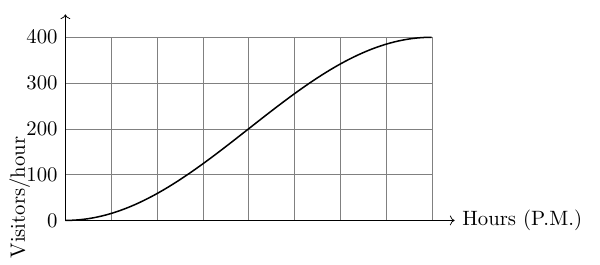
\includegraphics[width=0.6\linewidth]{data/calculus-figures/t8-tb19.png}\end{center}
\begin{list}{}{\setlength{\leftmargin}{3em}\setlength{\labelwidth}{2.5em}\setlength{\itemsep}{0pt}\setlength{\topsep}{2pt}}
\item[(A)] between 1 and 2 P.M.
\item[(B)] between 3 and 4 P.M.
\item[(C)] between 4 and 5 P.M.
\item[(D)] after 6 P.M.
\end{list}

\bigskip\noindent\textbf{TB20.}\ The velocity table is $\begin{array}{c|rrrrrr}t\text{ (sec)}&0&2&4&6&8&10\\\hline v(t)\text{ (units/sec)}&4&5&2&-2&-4&0\end{array}$. Use the five indicated trapezoids to estimate how far from its starting point the object is when it comes to rest at $t=10$.
\begin{list}{}{\setlength{\leftmargin}{3em}\setlength{\labelwidth}{2.5em}\setlength{\itemsep}{0pt}\setlength{\topsep}{2pt}}
\item[(A)] $0$ units
\item[(B)] $3$ units
\item[(C)] $6$ units
\item[(D)] $9$ units
\end{list}

\bigskip\noindent\textbf{TB21.}\ An 18-wheeler is traveling at a speed given by $v(t)=\dfrac{100(t+1)}{t+2}$ mph at time $t$ hours. The fuel economy for the diesel fuel in the truck is given by $f(v)=5+0.008v$ miles per gallon. The amount, in gallons, of diesel fuel used during the first 3 hours is approximately
\begin{list}{}{\setlength{\leftmargin}{3em}\setlength{\labelwidth}{2.5em}\setlength{\itemsep}{0pt}\setlength{\topsep}{2pt}}
\item[(A)] $20.5$
\item[(B)] $28.7$
\item[(C)] $33.2$
\item[(D)] $37.5$
\end{list}

\end{document}
